\section{\uppercase{Results}}
\label{sec:results}

\subsection{Axis Validation}
% Figure~\ref{fig:axis_validation} shows the drop of each axis under the controlled perturbations. The colour axis drops by 0.34, 0.66 and 0.96 for colour shifts of $\Delta E^*_{ab} = 5$, 10 and 20. Under the same perturbation, the other three axes change by at most 0.02. Blur lowers the texture score by 0.64 at $\sigma = 2$\,px and by 0.81 at $\sigma = 4$\,px. At $\sigma = 2$\,px colour and structure change by less than 0.05. Beyond $\sigma = 4$\,px the texture score does not drop further. However, the stronger blur starts to affect colour (0.26) and structure (0.28) as well. Structure drops by 0.28, 0.41 and 0.49 for displacements of at most 16, 32 and 64 pixels, while the texture and pattern change by at most 0.14. The colour, however, does appear to change by 0.22, 0.35 and 0.48 with increasing warping. 

\noindent The validation in Figure~\ref{fig:axis_validation} shows two dependencies between axes. First, the colour axis reacts to displacement almost as strongly as structure does (0.22 to 0.48 against 0.28 to 0.49). Colour is compared at small, fixed pixel regions. Consequently, when a stripe moves, the colour at those positions changes. Structure, on the other hand, does not react to a colour shift. Second, the pattern axis reacts to blur (0.40 to 0.48), because removing fine detail also changes the shape of the spectrum. We therefore read texture and pattern together and interpret a low colour score as either a different colour or a displaced region. Noise with a standard deviation of 0.05 changes no axis by more than 0.05. At 0.2, colour and pattern drop by 0.23 and 0.24 respectively. This indicates that these two axes are less reliable on very noisy estimates.

\begin{figure}[t]
  \centering
  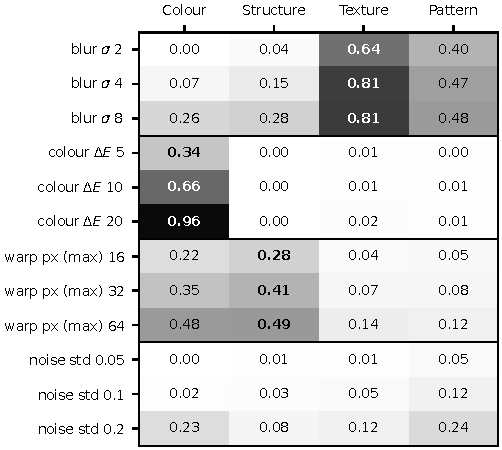
\includegraphics[width=\columnwidth]{figures/axis_specificity.pdf}
  \caption{Axis specificity: mean drop of each score under controlled perturbations of all 144 final images. Bold indicates which axis a perturbation targets.}
  \label{fig:axis_validation}
\end{figure}

\subsection{Order of Commitment Across Properties}
Figure~\ref{fig:curves_all} shows the mean curves of all six axes. In all three models, the pose and the coarse structure of the garment are fixed first. Texture, pattern and colour steadily improve throughout the sampling steps. The pose of the final image is present from step 1, meaning that the mean PCK with respect to the final skeleton is at least 0.95 from step 1 on in every model. The only exception is the estimate of IDM-VTON at step 0, which is close to pure noise and in which OpenPose often does not find a full skeleton (PCK 0.73). In every model, structure rises steeply in the first few steps, reaching 0.81 to 0.88 at step 10 and then increasing slowly until the last denoising step. 

\begin{figure*}[t]
  \centering
  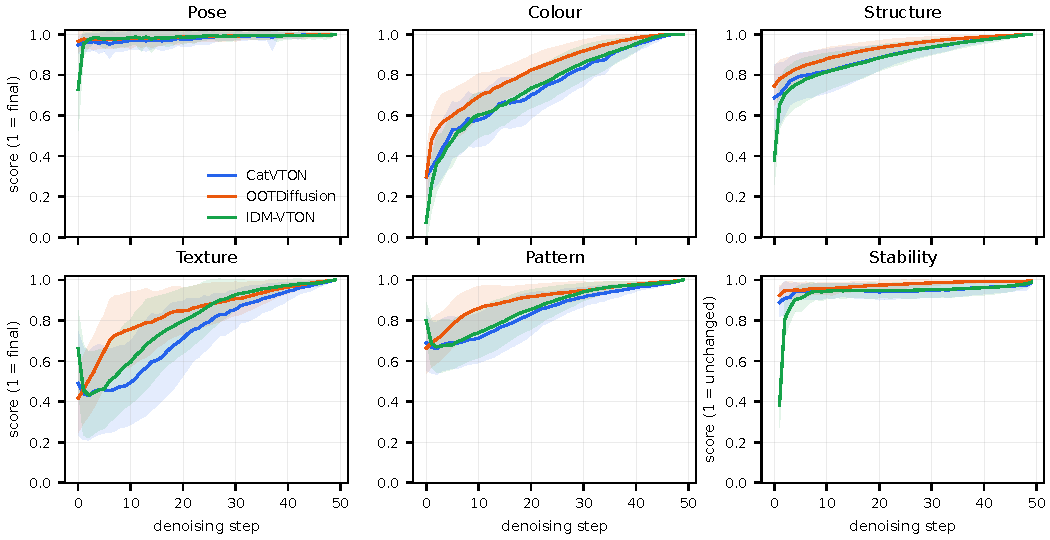
\includegraphics[width=\textwidth]{figures/curves_all.pdf}
  \caption{Per-step score of each axis, mean over the 48 pairs per model. The shaded band visualises $\pm 1$ standard deviation. Pose, colour, structure, texture and pattern are measured against the final frame of the same run, stability against the previous step.}
  \label{fig:curves_all}
\end{figure*}


\noindent Texture and pattern are resolved in a second phase. In CatVTON and IDM-VTON, the texture score first decreases from 0.49 to 0.44 in CatVTON and from 0.66 to 0.44 in IDM-VTON at step 3. These initial estimates contain a fair amount of noise. The estimate then becomes smooth. The texture score only rises again from around step 5 in IDM-VTON and step 10 in CatVTON. Colour rises at an almost constant rate until the last step, in CatVTON from 0.58 at step 10 to 0.83 at step 30 and in OOTDiffusion from 0.69 to 0.92. Since the band decomposition in Section~\ref{sec:res_bands} shows that chroma progresses as fast as luminance, however, this does not mean that the colour of the garment appears last. The colour axis requires most pixels to be within a small $\Delta E^*_{ab}$ of their final value and it also reacts to small displacements. Consequently, it keeps rising as long as regions are moving. The stability curves show that the estimate changes most in the first steps. After step 10, the step-to-step SSIM stays above 0.94 in every model, so the large changes happen early and are followed by many small corrections.
\\ \\
Figure~\ref{fig:x0_strip} shows an example with a striped garment. All three models settled the general layout and the shape of the top by step 5, but the stripes appear at different steps.
\\ 
\begin{figure}[t]
  \centering
  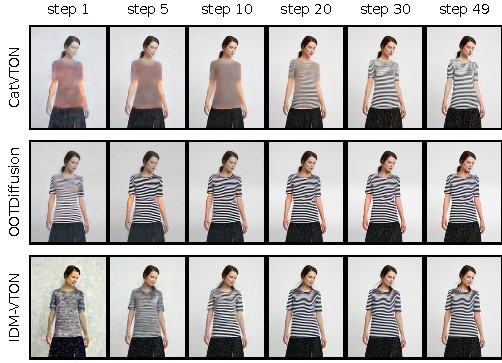
\includegraphics[width=\columnwidth]{figures/x0_strip.pdf}
  \caption{Decoded estimate $\hat{x}_0$ at six steps for one striped garment. \ootd shows the stripes from step 1, \idm from around step 5 and \catvton only from step 20.}
  \label{fig:x0_strip}
\end{figure}

\noindent Figures~\ref{fig:x0_strip_floral} and~\ref{fig:x0_strip_lettering} show two more examples. On the floral print, \ootd again shows the pattern from step 1, but \idm is now as late as \catvton: neither shows the flowers before step 20 and at step 5 \idm even shows horizontal stripes that are not in the garment. On the lettering, the large letters are readable by step 5 in all three models and only the small print below them appears later, between step 10 and 20.

\begin{figure}[t]
  \centering
  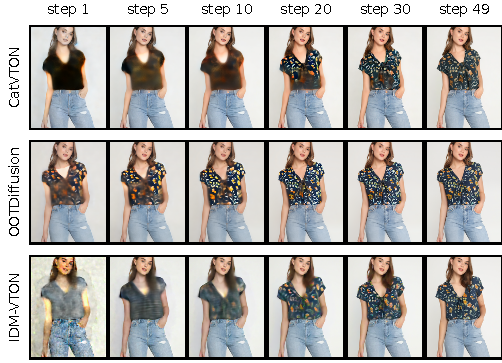
\includegraphics[width=\columnwidth]{figures/x0_strip_floral.pdf}
  \caption{Decoded estimate $\hat{x}_0$ for a floral print. \ootd shows the flowers from step 1, \catvton and \idm only from around step 20.}
  \label{fig:x0_strip_floral}
\end{figure}

\begin{figure}[t]
  \centering
  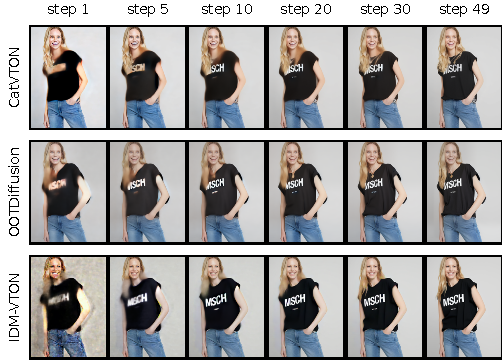
\includegraphics[width=\columnwidth]{figures/x0_strip_lettering.pdf}
  \caption{Decoded estimate $\hat{x}_0$ for a garment with large lettering. All three models show the lettering by step 5.}
  \label{fig:x0_strip_lettering}
\end{figure}

\subsection{Differences Between Models}
OOTDiffusion reaches its final state earlier than the other two models on every axis except pose, where all three are close to 1 from step 1. Its AUC is higher than that of both CatVTON and IDM-VTON for colour, structure, texture, pattern and stability ($p < 10^{-4}$ in every comparison, resulting from a paired Wilcoxon test over 48 pairs). The difference is most pronounced for texture and pattern. At step 10, the texture score of OOTDiffusion is 0.76, compared against 0.49 for CatVTON and 0.60 for IDM-VTON. Its pattern score is 0.86, against 0.71 and 0.74 respectively. CatVTON and IDM-VTON behave more similarly. Their colour AUC is nearly the same (0.749 and 0.751, $p = 0.92$). As suggested by LPH-VTON~\cite{liu2026lphvton}, CatVTON has a slightly higher structure AUC (0.894 against 0.883, $p = 0.01$), a weak indication that it is more structure-biased, while IDM-VTON has a higher texture AUC (0.801 against 0.743, $p < 10^{-3}$), making it more texture-biased. The lowest stability AUC was observed for IDM-VTON (0.935), primarily caused by the large change between step 0 and step 1 (SSIM 0.38). OOTDiffusion appears to be the most stable model. Its early commitment is not followed by extra compensation corrections later. None of these differences in timing shows up in the final images, whose FID and KID are almost the same for the three models (Table~\ref{tab:models}).

\subsection{Differences Between Garment Categories}
Figure~\ref{fig:summary_auc} gives the AUC per category, Figure~\ref{fig:curves_by_category} the mean curve per category for each model. Garments with large uniform areas (solid, lettering, graphic and structural) have a high structure AUC between 0.91 and 0.95 in every model, against 0.82 to 0.93 for the four repeating patterns (stripe, floral, dot and check). The Kruskal--Wallis test over the eight categories indicates that the difference between them is significant for structure in all three models ($p < 0.005$). This can already be observed at step 10. The uniform garments reach a structure score of 0.85 to 0.91 in CatVTON and IDM-VTON, the repeating patterns 0.73 to 0.79. In OOTDiffusion the gap is smaller, namely 0.89 to 0.93 against 0.84 to 0.88.
\\ \\
Texture exhibits the largest differences between both categories and models. In CatVTON, the texture score of stripes stays around 0.28 for the first ten steps and only rises steeply from about step 15. The floral and dot prints show a similar but smaller delay; 0.37 and 0.38 at step 10, compared to 0.73 for lettering. IDM-VTON shows the same delay for floral and dot prints; 0.36 and 0.38 at step 10, compared to 0.78 for lettering, but resolves stripes much earlier than CatVTON (0.66). In both models, the texture scores at step 10 differ by more than 0.4 between categories ($p < 0.005$) and the pattern scores by 0.24 to 0.28 ($p < 0.002$). In most categories, OOTDiffusion's texture curves rise in the first ten steps and lie close together. Floral prints are the exception: their texture score stays almost constant between step 10 and 30 and only then rises again.
\\ \\
The categories return similar results across models. The largest difference between models is observed for stripes. The texture AUC of CatVTON on stripes is 0.61, its lowest of all categories, against 0.83 and 0.91 for IDM-VTON and OOTDiffusion respectively. Its pattern AUC (0.79 against 0.88 and 0.93) and colour AUC (0.70 against 0.74 and 0.82) follow the same trend, which matches the example given in Figure~\ref{fig:x0_strip}. Colour differs less between categories: the AUC varies by 0.09 to 0.13 within a model. Only for CatVTON is this difference significant ($p = 0.02$). Lettering has the highest colour AUC in every model (0.81 to 0.87). It is worth noting that each category only contains six pairs, so these per-category results are means over a small number of garments.

\begin{figure*}[t]
  \centering
  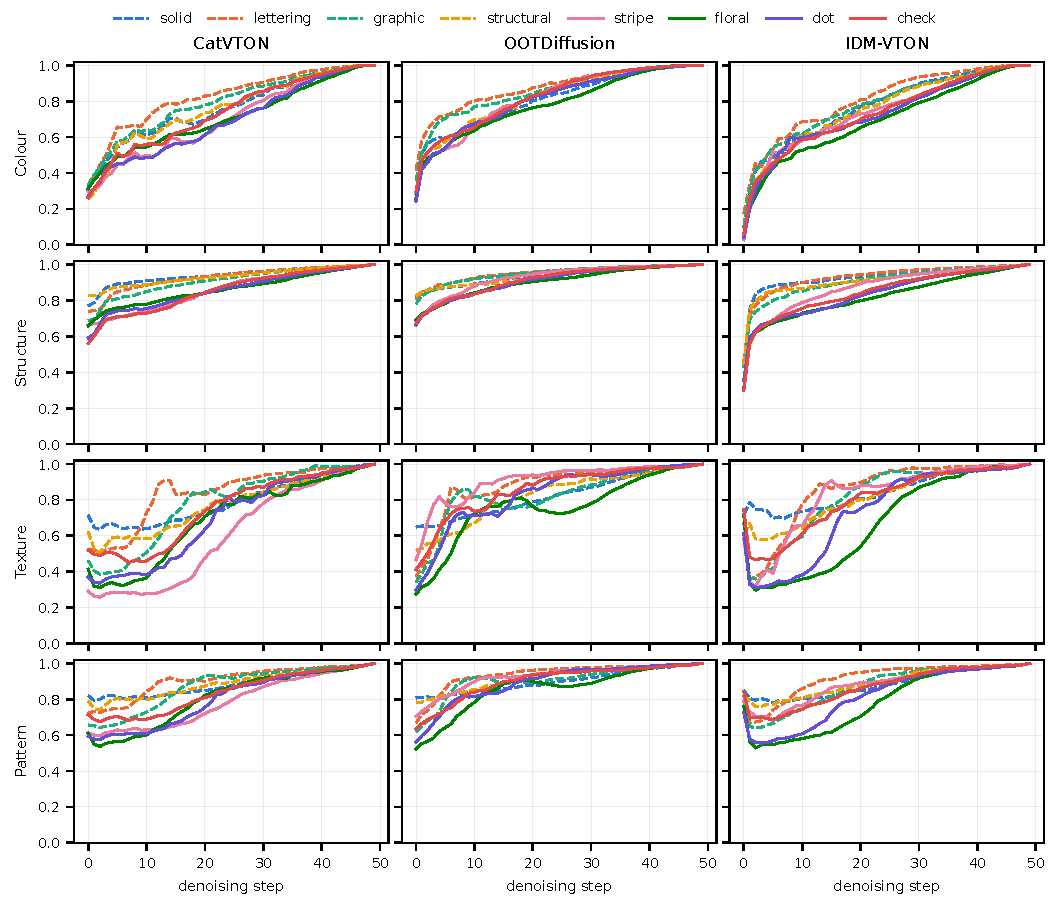
\includegraphics[width=\textwidth]{figures/curves_by_category.pdf}
  \caption{Mean per-step score of the four garment axes per category. Dashed lines are garments with large uniform areas, solid lines indicate repeating patterns.}
  \label{fig:curves_by_category}
\end{figure*}

\begin{figure*}[t]
  \centering
  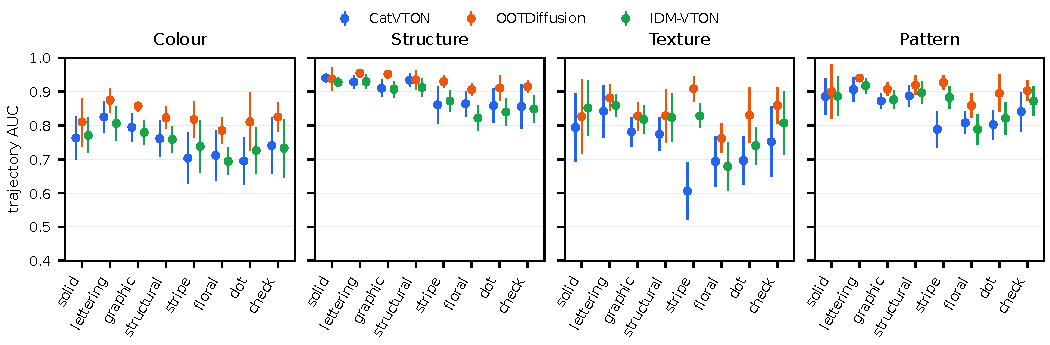
\includegraphics[width=\textwidth]{figures/summary_auc.pdf}
  \caption{Trajectory AUC of the four garment axes per category and model. Values are the mean over six pairs, with whiskers indicating $\pm 1$ standard deviation. Pose and stability are close to 1 in every category and are omitted.}
  \label{fig:summary_auc}
\end{figure*}

\subsection{Coarse-to-Fine Generation}
\label{sec:res_bands}
Figure~\ref{fig:band_progress} shows the progress of the three frequency bands. All three models generate the garment from coarse to fine. The coarse-to-fine index is positive in all 48 pairs for every model ($p < 10^{-14}$ against zero), with a median of $+0.46$ for CatVTON, $+0.43$ for IDM-VTON and $+0.30$ for OOTDiffusion. In CatVTON and IDM-VTON, the coarse band reaches half of its progress after approximately 10 steps, while the fine band changes little until the last third of the trajectory. OOTDiffusion is less coarse-to-fine than the other two models ($p < 10^{-8}$ against both), while CatVTON and IDM-VTON do not contrast significantly ($p = 0.07$). This is not because OOTDiffusion resolves the coarse band later given that its coarse AUC (0.64) is close to that of CatVTON (0.67). The difference lies in the fine band, which progresses almost linearly from the start in OOTDiffusion (fine AUC 0.34, against 0.22 for CatVTON and 0.29 for IDM-VTON).

\begin{figure*}[t]
  \centering
  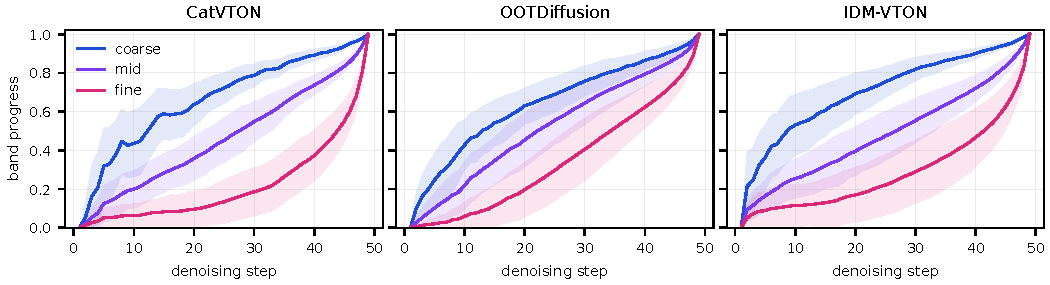
\includegraphics[width=\textwidth]{figures/band_progress.pdf}
  \caption{Progress of the coarse, mid and fine spatial-frequency bands towards the final frame, each normalised by its own distance at step 1 (mean over 48 pairs, $\pm 1$ standard deviation).}
  \label{fig:band_progress}
\end{figure*}
\vspace{\baselineskip}
\noindent In OOTDiffusion and IDM-VTON, luminance and chroma progress at the same rate; the median luminance-before-chroma indices ($+0.02$ and $+0.03$) do not differ significantly from zero. CatVTON resolves chroma before luminance in $79\%$ of the pairs (median index $-0.09$, $p < 10^{-4}$). Therefore, in CatVTON the colour of the garment is in place before its shading and fine structure.
